\pdfoutput=1

\documentclass[11pt,a4paper]{article}
\renewcommand\thesection{\Alph{section}}
\renewcommand\thesubsection{Séance \arabic{subsection}}
\renewcommand\thesubsubsection{\thesection-\arabic{subsubsection}}
\usepackage[a4paper, total={6.5in, 10in}]{geometry}
\usepackage{setspace}
\doublespacing

\usepackage[bf,pagestyles,raggedright]{titlesec}
\titlespacing*{\section}{-40pt}{5.5ex plus 1ex minus .2ex}{1.5ex plus .2ex}
\titlespacing*{\subsection}{-30pt}{3.25ex plus 1ex minus .2ex}{1.5ex plus .2ex}
\titlespacing*{\subsubsection}{-30pt}{3.25ex plus 1ex minus .2ex}{0.5ex plus .2ex}
\titleclass{\part}{top}
\titleformat{\part}[block]{}{}{0pt}{\thispagestyle{fancy}\centering\Huge\bfseries}

\usepackage{lastpage}
\usepackage{fancyhdr}
\pagestyle{fancy}
\fancyhf{}
\setlength{\headheight}{13.6pt}
\fancyhead[L]{\leftmark\hfill\today}
\fancyfoot[C]{p. \thepage/\pageref{LastPage}}
\renewcommand{\footrulewidth}{0.3pt}

\usepackage[titles]{tocloft}
\addtolength{\cftsecnumwidth}{15pt}

\title{\Huge\bfseries Cours }

\author{\large Mael GOODALL}
\date{\large\today}
\usepackage{graphicx}
\graphicspath{{images/}}
\usepackage{mathrsfs}
\usepackage{amsfonts}
\usepackage{amsmath}
\usepackage{amssymb}
\usepackage{hyperref}

\newif\ifdraft
\draftfalse

\begin{document}

\newgeometry{top=-0.2in}
\maketitle
\tableofcontents
\thispagestyle{fancy}
\restoregeometry


\part{suivie séance}
	\setcounter{subsection}{2}
	\subsection{}
		\subsubsection{recherches : }
			these en 180s moteur thermoacoustique (interet limiter)\\
			introduction à la thermoacoustique M1 : \href{https://perso.univ-lemans.fr/~gpenelet/enseignement/support_cours/poly_thermoac.pdf}{there}\\
			p.8 diagrame de clapeyron d'un cycle sur pour une onde acoustique stationaire sur une paroi soumise à un gradien de température.\\
			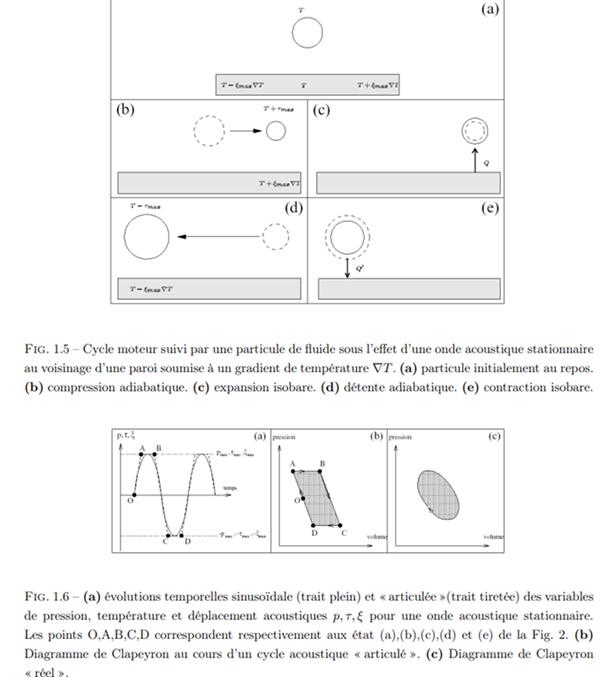
\includegraphics{p_8_intro_M1.png}\\
			Convertion d'énèrgie dù à un retard entre les dù à une petite distance à la paroi...\\
			voir p.9
	\subsection{}
		p.22
	\subsection{}
		fin lecture partie 1\\
		rechercher et \emph{noter} ordres de grandeurs pour experiences.
	\subsection{}
		p.37 flux de chaleur moyen.
	\subsection{}
		these sur le sujet (avec montage réalisable p.70) \href{file:///home/tamary/Downloads/th%C3%A8se%20r%C3%A9frig%C3%A9rateur%20thermoacoustique%20-%20Biblioth%C3%A8que%20Ecole%20Centrale%20....pdf}{there}\\
		materiel nécéssaire : 
		\begin{itemize}		
			\item tube PVC (goutiere ou autre) (isolation thermique un peu, sonore idéalement ?)
			\item haut parleur (20 à 100 W)
			\item micro (detecter pression pic a pic)
			\item thermometre entre deux points (début et fin du stack)
			\item bouchon fin de tube
			\item stack (plaque de 1 à 10cm de long / ordre de diametre tube large / ordre de 0.1mm epaisseur)
		\end{itemize}
		
	\subsection{}
		fabrication du stack/refrigirateur \href{https://www.acs.psu.edu/drussell/publications/thermodemo.pdf}{there}\\
		\[\delta_k=\sqrt{\frac{\kappa}{\pi f\rho c_p}}\simeq \frac{2.4 * 10^{-3}}{\sqrt{f}}\]
		dans les conditions normales 
		
	\subsection{}
		demande de materiaux au labo
		
		materiaux stack (objectif faible conductivité (mais élevée devant air $\kappa=0.026$W/m.K) et capacité thermique élevée voir 
		\href{https://perso.univ-lemans.fr/~gpenelet/enseignement/support_cours/poly_thermoac.pdf}{p.19}) : 
		\begin{itemize}		
			\item papier : $\kappa=0.05-0.2$ W/m.K ; $c=1.4$ kJ/kg.K faible conductivité thermique mais peu rigide
			\item acier inoxydable : $\kappa=15-25$ W/m.K ; $c=0.5$ kJ/kg.K mais difficile à trouver et à construire le stack.
			\item plastique : $\kappa=0.1-0.5$ W/m.K ; $c=1-2$ kJ/kg.K
			\item  cuivre : $\kappa=390$ W/m.K ; $c=0.39$ kJ/kg.K
		\end{itemize}
		
	\subsection{}
		utilité accéléromètre
		préparation à faire :
		\begin{itemize}		
			\item construire stack (dimension résonateur)
			\item installer stack dans résonnateur
			\item installer micro (mesure pression) au niveau du haut parleur
			\item installer thermocouple (différentiel de température) aux bords du stack
			\item accéléromètre (mesure de vitesse) sur le haut-parleur
			\item carte d'aquisition des données
			\item mesurer la température extèrieur
			\item faire en sorte que le haut-parleur envoie une onde plane (ex : plaque acroché au bout de la membrane)
			\item relier résonnateur et haut-parleur
		\end{itemize}
		
	\subsection{}
		début de la fabrication du système de mesure
		diamètre tube 45mm
		liste materiel :
		\begin{itemize}		
			\item 2 thermocouple (mesure différentielle)
			\item 1 micro
			\item 1 acceleromètre 
			\item 1 carte d'acquisition (au moins 3 ports)
			\item 1 haut-parleur 
			\item tube diamètre 45mm
		\end{itemize}
		
	\subsection{}
		test et mise en place de l'aquisition (micro + thermocouple)\\
		sortie thermocouple : variation de l'ordre du $\mu$m (trop faible même pour oscilo sans amplification)\\
		regarder pour amplificateur (résist)\\
		micro : 1.5V à 261Hz (pic de fonctionnement haut parleur)\\
		
	\subsection{}
		taille du tube $\emptyset=49mm$, 564mm de longueur.\\
		longueur d'onde pour 1 onde stationnaire : $f=\frac{c}{\lambda}$\\
		d'après le modèle du gaz parfait (wiki) $c=20.05\sqrt{T}$\\
		ici $T=23 \quad\text{to}\quad 24.5 ^\circ C$ donc $c= 345.5$m.s$^{-1}$\\
		donc pour 1 longueur d'onde de la taille du tube : $f_1= 613$Hz\\
		Shéma du montage : \\
		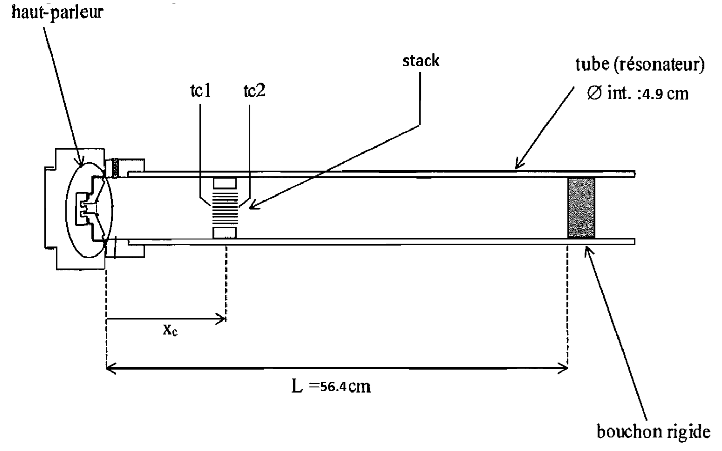
\includegraphics{shema_montage.png}
	\subsection{}
		coeficients obtenus pour mesure1 : [-1.37424721  1.18577569 -0.01010258]
		$\delta_k =84\mu$m
		
	\subsection{}
		Voir sonde température arduino\\
		tube $\emptyset=45$mm et 891mm de long\\
		p70 de la these : déphasage pression-vitesse acoustique \\
		
		\href{https://matmake.com/materials-data.html}{materials data} et 
		\href{https://en.wikipedia.org/wiki/List_of_thermal_conductivities}{wikipedia conductivities} et 
		\href{https://en.wikipedia.org/wiki/Table_of_specific_heat_capacities}{wikipedia capacité}: 
		\begin{itemize}		
			\item plexiglass : $\kappa=0.18 \quad W.m^{-1}.K^{-1}$ ; $c=1.45$ kJ/kg.K
			\item wood : $\kappa=0.04-0.12 \quad W.m^{-1}.K^{-1}$ ; $c=1.7$ kJ/kg.K
		\end{itemize}
	\subsection{}
		fichier svg pour differents stacks tests de découpe laser sur plexiglass.
	\subsection{}
		protocole expérimental :
		\begin{itemize}		
			\item stacks avec differentes tailles de maille et différentes épaisseurs.
			\item différents points de mesures.
			\item faire des mesures en csv 
			\item faire les graphs
		\end{itemize}
		voir page 77 thèse pour la position du stack.\\
		sonde de température tout les cm entre 13 et 18\\
		trous de 5mm de diamètre 
	\subsection{}
		thermomètre : LM335A//
		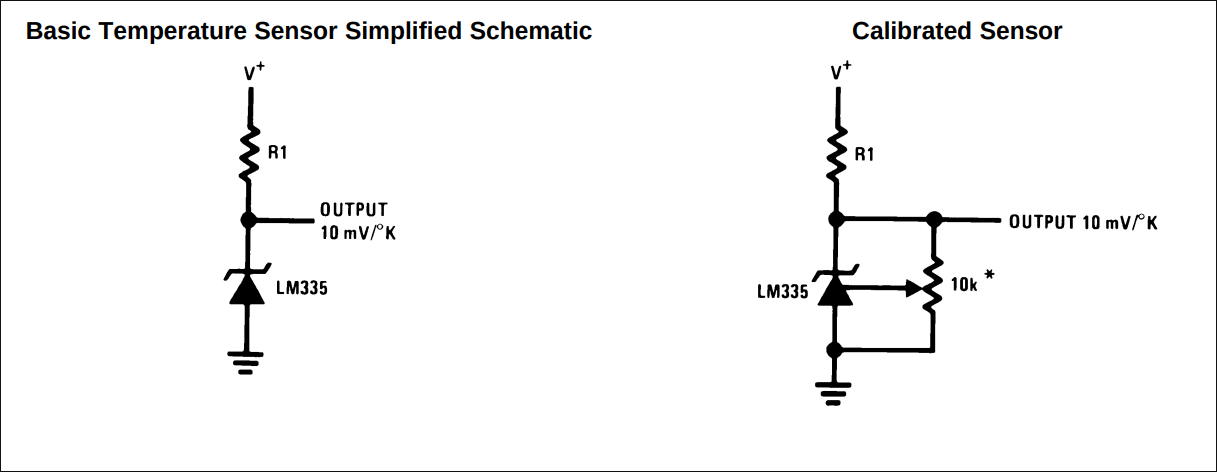
\includegraphics{shema_elec.png}
		forward current : 1mA\\
		durée d'acquisition 5s, 2000 points
		montage : \\
		sans calibrage : -2.624/-2.597/-2.63/-2.648/-2.614\\
		avec : -2.65/-2.623/-2.611/-2.498/-2.615\\
		mieux sans calibrage (écart type 20\% plus faible)
	\subsection{}
		position 2 et 5 613Hz durée : 1min sans son, 2min avec 20VPP
	\subsection{}
		testes (voir latis pro)
	\subsection{}
		pour mesurer la fréquence de résonnance, on produit un bruit blanc et on cherche les pics dans la transformée de fourier.\\
		on cherche la meilleure position pour le stack avec une vérification de la fréquence à chaque fois 5min de mesure à chaque fois.\\
		on mesure la différence de température à vide sur 10/20min. sans le stack/avec.
		\end{document}
